% BevoTag Project Definition, memo-style report.
% Formatting follows Writing-Guides/ECE Style Guide.pdf and Writing-Guides/Template for Memo Style Reports.doc.
% Build: pdflatex main.tex (twice), e.g. with TinyTeX in WSL Ubuntu-22.04.
\documentclass[12pt,letterpaper]{article}

\usepackage[T1]{fontenc}
\usepackage{newtxtext,newtxmath}              % 12-pt Times
\usepackage[margin=1in]{geometry}             % 1-in margins on all sides
\usepackage{setspace}
\setstretch{1.43}                             % Word "1.5 lines" for 12-pt Times (20.7-pt baselines)
\usepackage[document]{ragged2e}               % do not justify the right margin
\usepackage{graphicx}
\usepackage{xcolor}
\usepackage{array,tabularx,booktabs}
\usepackage{enumitem}
\usepackage{caption}
\usepackage{float}
\usepackage{placeins}
\usepackage{etoolbox}
\usepackage{tikz}
\usetikzlibrary{arrows.meta,positioning,fit,calc}
\usepackage[nobottomtitles*]{titlesec}        % never leave a heading on the last line of a page
\usepackage[hidelinks]{hyperref}
\usepackage{url}
\renewcommand{\UrlFont}{\normalfont}
\def\UrlBreaks{\do\/\do\-\do\.\do\_\do\=\do\?}

% Block paragraphs: no indentation, one empty line between paragraphs.
\setlength{\parindent}{0pt}
\setlength{\parskip}{\baselineskip}
\renewcommand{\bottomtitlespace}{0.08\textheight}

% Ragged-right text without hyphenated line breaks.
\hyphenpenalty=10000
\exhyphenpenalty=10000

% Headings (Style Guide 2.3): one empty line before, text starts on the next line, no numbers.
%   1st level: ALL CAPS, bold   2nd level: Initial Caps, bold   3rd level: Initial Caps, bold italic
\setcounter{secnumdepth}{0}
\titleformat{\section}{\normalfont\bfseries}{}{0pt}{\MakeUppercase}
\titleformat{\subsection}{\normalfont\bfseries}{}{0pt}{}
\titleformat{\subsubsection}{\normalfont\bfseries\itshape}{}{0pt}{}
\titlespacing*{\section}{0pt}{0pt}{-\parskip}
\titlespacing*{\subsection}{0pt}{0pt}{-\parskip}
\titlespacing*{\subsubsection}{0pt}{0pt}{-\parskip}

% Captions (Style Guide 2.4): bold, centered, "Table 1." above tables, "Figure 1." below figures.
\captionsetup{font={normalsize,bf},labelfont=bf,labelsep=period,justification=centering,singlelinecheck=false}
\captionsetup[table]{position=above,skip=6pt}
\captionsetup[figure]{position=below,skip=6pt}
% A graphic follows the paragraph that introduces it, or tops the next page, and never floats
% past the next heading (Style Guide 2.4).
\renewcommand{\topfraction}{0.9}
\renewcommand{\bottomfraction}{0.8}
\renewcommand{\textfraction}{0.07}
\renewcommand{\floatpagefraction}{0.9}
\setcounter{topnumber}{3}
\setcounter{totalnumber}{4}
% One empty line between a graphic and the text around it.
\setlength{\textfloatsep}{\baselineskip}
\setlength{\floatsep}{\baselineskip}
\setlength{\intextsep}{0.5\baselineskip}
\setlength{\emergencystretch}{3em}

% Indented lists that continue the preceding paragraph (Style Guide 2.5).
\setlist[itemize]{leftmargin=0.5in,topsep=0pt,itemsep=0pt,parsep=0pt}

% Single-spaced 12-pt tables.
\newcolumntype{L}[1]{>{\RaggedRight\arraybackslash}p{#1}}
\newcolumntype{Y}{>{\RaggedRight\arraybackslash}X}
\newenvironment{spectable}{\setstretch{1.0}\renewcommand{\arraystretch}{1.1}}{}

% Page numbers centered at the bottom, on every page but the first.
\pagestyle{plain}

\pretocmd{\section}{\FloatBarrier}{}{}
\begin{document}
\thispagestyle{empty}

%----------------------------------------------------------------------------------------------------
% MEMO HEADING (Style Guide 2.2): bold field titles, two columns, single spacing within a field,
% 1.5 spacing between fields.
%----------------------------------------------------------------------------------------------------
\begingroup
\setstretch{1.0}
\newcommand{\fieldgap}{\\[6.2pt]}
\noindent\begin{tabular}{@{}p{1.1in}@{}p{\dimexpr\linewidth-1.1in\relax}@{}}
\textbf{DATE:} & October 15, 2026 \fieldgap
\textbf{TO:} & Dr.\ Haris Vikalo \\ & Mugdha Jadao \fieldgap
\textbf{FROM:} & Ethan Chua \\ & Esteban Martinez \\ & Li Shi \\ & Andrew Yin \\ & Abhirit Das \fieldgap
\textbf{SUBJECT:} & Project Definition for BevoTag, an Open Asset-Tracking Tag for the UT Austin Campus \\
\end{tabular}
\endgroup

%----------------------------------------------------------------------------------------------------
\section{Introduction}
%----------------------------------------------------------------------------------------------------
This Project Definition defines the design problem that the BevoTag team will solve in Senior
Design and explains how the five-member team has organized itself to solve it. BevoTag is a small
tag that a student or staff member attaches to a laptop, bag, or piece of university equipment to
locate it anywhere on the University of Texas at Austin campus. Satellite positioning such as GPS
fails inside buildings, and consumer tags such as the Apple AirTag update an item's location only
when a nearby phone from the same manufacturer detects them \cite{airtag}. BevoTag is open in the
sense that it needs no manufacturer's phone network: it estimates the item's position from the
Wi-Fi networks already installed across campus and from its own motion sensor, and it reports that
position to its owner on a campus map. In short, the team will build a tag, firmware, a building
survey, and an application that together place an item within a median of 5~m and in the correct
room in more than 90\% of trials.

The design problem is to track an item continuously, indoors and outdoors, without new
infrastructure. Wi-Fi measurements alone can mislocate a device by several meters because signals
fluctuate as the environment changes, and a low-cost motion sensor alone drifts by tens of meters
within a minute; combining the two lets each correct the other. The project will test this approach in surveyed areas beginning with
the Engineering Education and Research Center (EER). Wi-Fi, radio-emission, data-security, and
battery-safety standards constrain the design, as does university network policy. The team
commits to recording no one's network traffic, to encrypting and limiting location data, and to
using the campus network only as an ordinary client.

The requirements turn this need into measurable targets. Beyond the accuracy targets, the system
must update an item's location at least every 10~s while it moves and run at least 24~h on one
battery charge. Two sub-teams will meet these targets: Esteban Martinez and Li Shi will build the
tag hardware and firmware, and Andrew Yin and Abhirit Das will build the localization software and
the user application, with Ethan Chua coordinating as Project Lead. The team communicates on
Discord, tracks every task on GitHub, reviews all code and writing before submission, and decides
contested questions by majority vote after testing the options.

%----------------------------------------------------------------------------------------------------
\section{Problem Statement}
%----------------------------------------------------------------------------------------------------
BevoTag must locate a tagged item to within a few meters across indoor and outdoor areas of campus
while relying only on existing campus Wi-Fi and its own motion sensor. Buildings block and reflect
satellite signals \cite{yoder}, and low-cost motion sensors drift \cite{imu}, so no single source
of position is reliable on its own. The Design Problem Description shows that fusing Wi-Fi
fingerprints with motion sensing meets this need within the limits that standards and ethical
obligations set. The Requirements Specification then turns that need into measurable targets, led
by a median position error under 5~m.

\subsection{Design Problem Description}
A successful BevoTag design must estimate an item's location indoors and outdoors without
infrastructure the team cannot control, and it must show that location to the item's owner on a
map. Existing trackers fail this need because satellite signals do not reach indoors and
crowdsourced tags depend on passing phones. BevoTag addresses the need by fusing Wi-Fi fingerprints
with motion sensing, an approach that brings three main challenges: limited power on the tag,
radio signals that change from moment to moment, and sensor drift. Because the tag reports
location, the design must also satisfy radio, data-security, and battery-safety standards and
protect the privacy of bystanders and owners.

\subsubsection{The Need for On-Campus Item Tracking}
Students, faculty, and staff need a way to find misplaced items anywhere on the main UT Austin
campus, known as the Forty Acres. Laptops, bags, and shared university equipment move between
classrooms, labs, libraries, and outdoor plazas many times a day, and an item left behind can be
anywhere among dozens of multistory buildings. A useful tracker must therefore work indoors, on any
floor, and in the narrow outdoor spaces between tall buildings. The team's goal is tracking that
needs neither new infrastructure, such as beacons installed in every building, nor a passerby who
owns a particular brand of smartphone.

\subsubsection{Why Existing Solutions Fall Short}
Three existing approaches to tracking fail on campus for different reasons. Satellite positioning
cannot reach indoors, crowdsourced Bluetooth tags stop updating when no compatible phone passes
by, and Wi-Fi positioning based on signal strength alone errs by enough to place an item in the
wrong room.

Satellite positioning fails indoors and degrades between tall buildings. Global Navigation
Satellite Systems (GNSS), the family of satellite positioning systems that includes GPS, compute
a receiver's position from faint signals broadcast by satellites about 20,200~km above the Earth
\cite{gps}. Walls and roofs block those signals. Between tall buildings, signal blockage and
multipath, the arrival of signals only after they reflect off nearby walls, degrade GNSS so much
that earlier low-cost urban systems reported position errors greater than 9~m
\cite[Sec.~1.1.1]{yoder}.

Crowdsourced tags locate an item only when a compatible phone happens to pass nearby. The Apple
AirTag and the Samsung Galaxy SmartTag broadcast a short-range Bluetooth signal, and nearby phones
from the same manufacturer detect that signal and report its location \cite{airtag},
\cite{smarttag}. In an empty lab at night no such phone passes by, so the tag's location stops
updating until one does.

Wi-Fi positioning based only on signal strength is too coarse for room-level tracking. These
systems estimate position from the received signal strength indicator (RSSI), a measure of how
strong each nearby Wi-Fi signal is when it reaches the device. Signal strength fluctuates as the
environment changes \cite{hechan}, so RSSI fingerprinting typically locates a device only to
within 1 to 5~m \cite[Table~4]{rssi}, which can place it in the wrong room.

\subsubsection{Theory of Operation}
BevoTag combines two sources of position information whose errors differ: campus Wi-Fi
measurements, which are noisy but do not drift, and a motion sensor, which is smooth over short
periods but drifts. A fusion algorithm uses each source to correct the other. The final design may
compute this estimate on the tag or on a server; the team will decide after measuring the
prototype hardware, as the Design Challenges explain.

Wi-Fi measurements locate the tag by matching them against a survey of each building. UT Austin
operates campus Wi-Fi networks, including utexas-iot, which serves Internet of Things devices
once their owners register each device's hardware address \cite{utiot}. In addition to RSSI, some
Wi-Fi chips report channel state information (CSI), the frequency response of each of dozens of
narrow sub-channels, which describes how much the signal on each sub-channel is weakened and
delayed along its path \cite{espcsi}. Walls, furniture, and room
geometry shape these values, so CSI acts as a detailed fingerprint of a location. The team will
first survey a building by recording Wi-Fi measurements at many points whose positions it knows.
The system can then estimate the tag's position by finding the survey points whose measurements
best match the tag's current measurements.

A motion sensor tracks the tag between Wi-Fi fixes but drifts when used alone. An inertial
measurement unit (IMU), similar to the sensor that rotates a smartphone's screen, measures
acceleration along three axes and rotation about them. Adding up these measurements from a known
starting point, a technique called dead reckoning, tracks the tag's movement many times per
second. Small sensor errors accumulate, however, so the estimate drifts farther from the truth the
longer it runs: a simple low-cost inertial system can accumulate more than 150~m of average
position error within 60~s \cite{imu}.

A fusion algorithm combines the two sources so that the result neither jumps like Wi-Fi alone nor
drifts like the IMU alone. A standard candidate is the extended Kalman filter (EKF)
\cite{welch}, which uses the IMU to predict how the tag has moved and uses each new Wi-Fi fix to
correct the accumulated drift, weighting each source by how reliable it currently is. Outdoors, where satellite signals are
available, the same algorithm can also accept a GNSS position as an optional third source.

\subsubsection{Design Functionality and Scope}
BevoTag is a system of a tag, a location server, and a user application that together turn Wi-Fi
and motion measurements into a position on a campus map. The project covers a working prototype
tested in surveyed areas starting with EER. It excludes cellular connectivity, a campus-wide
survey, mass-production tooling, and the tracking of people.

Figure~\ref{fig:overview} on the next page shows how the parts of the system work together. The tag measures nearby
Wi-Fi signals and its own motion (step~1) and sends these measurements over the campus Wi-Fi
network to the location server (step~2). The server combines them with a previously recorded
survey of the building to estimate the tag's position, or it receives an estimate that the tag
computed itself (step~3). The user application then displays that position on a campus map
(step~4). To deliver this behavior, any BevoTag design must perform four functions:
\begin{itemize}
  \item \textbf{Wi-Fi measurement:} record the RSSI and, where the hardware supports it, the CSI
    of signals from nearby campus access points in the 2.4~GHz band.
  \item \textbf{Motion tracking:} sample the IMU's acceleration and rotation fast enough to follow a
    walking person carrying the tag.
  \item \textbf{Position estimation:} fuse the motion data with Wi-Fi position fixes, correcting the
    drift that accumulates in the motion estimate.
  \item \textbf{Reporting:} send the latest position and device status to an application that the
    owner can view.
\end{itemize}

\begin{figure}[!htp]\setstretch{1.0}
\centering
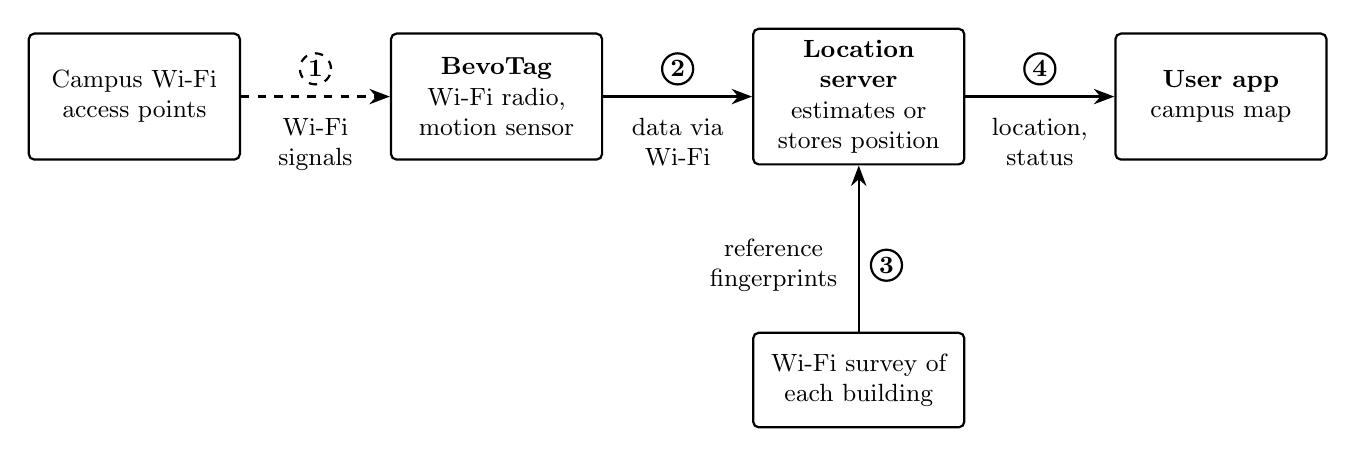
\begin{tikzpicture}[
    font=\small, >={Stealth[length=2.6mm]},
    blk/.style={draw, thick, rounded corners=2pt, align=center, minimum height=1.6cm,
                text width=2.4cm, inner sep=4pt},
    stepnum/.style={circle, draw, thick, fill=white, inner sep=1.2pt, font=\small\bfseries},
    lbl/.style={align=center, font=\small}]
  \node[blk] (ap)  at (1.35,0)   {Campus Wi-Fi\\access points};
  \node[blk] (tag) at (5.95,0)   {\textbf{BevoTag}\\Wi-Fi radio,\\motion sensor};
  \node[blk] (srv) at (10.55,0)  {\textbf{Location\\server}\\estimates or\\stores position};
  \node[blk] (app) at (15.15,0)  {\textbf{User app}\\campus map};
  \node[blk, minimum height=1.2cm] (map) at (10.55,-3.6) {Wi-Fi survey of\\each building};
  \draw[->, thick, dashed] (ap) -- node[stepnum, above=4pt] {1} node[lbl, below=4pt] {Wi-Fi\\signals} (tag);
  \draw[->, thick] (tag) -- node[stepnum, above=4pt] {2} node[lbl, below=4pt] {data via\\Wi-Fi} (srv);
  \draw[->, thick] (srv) -- node[stepnum, above=4pt] {4} node[lbl, below=4pt] {location,\\status} (app);
  \draw[->, thick] (map) -- node[pos=0.4, stepnum, right=4pt] {3}
                            node[pos=0.4, lbl, left=4pt] {reference\\fingerprints} (srv);
\end{tikzpicture}
\caption{How BevoTag Locates a Tagged Item}
\label{fig:overview}
\end{figure}

The project includes a working prototype tag, its firmware, a Wi-Fi survey of designated test
areas, and a user application. The tag will combine a Wi-Fi chip that can report CSI, such as the
ESP32-S3 \cite{espcsi}, with a low-noise IMU on a development board or a custom circuit board. Its
firmware will read the sensors and either process the measurements or send them to the server. The
survey will begin with EER and its adjacent outdoor plazas, and the application will display the
tag's position on a campus map.

Four related capabilities fall outside the project's scope. The tag will not use a cellular
connection such as LTE-M or NB-IoT, because these require a paid data plan and a second radio that
would raise cost and power consumption, and campus Wi-Fi already covers the target areas. The team
will not survey every building on campus, because a survey requires walking each floor and
recording measurements at many points. It will instead test in a few defined benchmark areas and
document the survey method so that others can add buildings later. The team will 3D-print or buy
the prototype enclosure rather than design it for injection molding, since the goal is a working
proof of concept rather than a manufacturable product. Finally, BevoTag locates objects, not
people, and the design excludes features meant to follow a person, such as continuous covert
tracking.

\subsubsection{Design Challenges}
Three challenges will most strongly shape the design: deciding where to compute the position,
coping with radio signals that never repeat exactly, and correcting motion-sensor drift quickly
enough. Each challenge requires a measurement on prototype hardware before the team can finalize
the design.

The first challenge is deciding whether to compute the position on the tag or on the server.
Processing CSI and running a fusion filter on a small microcontroller strains its memory and
battery. Sending raw measurements to the server moves that work off the tag but keeps the radio on
longer, which also drains the battery. The team will settle this trade-off by measuring CSI capture
rates, IMU data rates, and power draw on the prototype.

The second challenge is that indoor radio signals vary from moment to moment. The Wi-Fi
measurements recorded at a given spot fluctuate with noise and with changes in the environment,
such as people walking through hallways \cite{hechan}, so the matching method must tolerate
measurements that never exactly repeat the survey. The team will therefore record survey measurements at
several times of day and test the matching method on data that it did not use to build the survey.

The third challenge is correcting IMU drift before it grows large. Low-cost motion sensors
accumulate tens of meters of position error within a minute \cite{imu}, so Wi-Fi fixes must arrive often enough, and
be reliable enough, to keep the fused estimate from diverging from the true position. This
requirement ties the Wi-Fi update rate directly to the accuracy targets in the Performance
Specifications.

\subsubsection{Relevant Standards}
Six standards and policies constrain how BevoTag uses the radio spectrum, connects its sensors,
protects its data, powers itself, and uses the campus network. Their most direct effects are that
the tag must use a Wi-Fi chip that exposes CSI, a pre-certified radio module, encrypted telemetry,
and a certified, protected lithium battery. Appendix~A lists the specific clauses of each standard,
how each affects the design, and how the team will verify compliance.

IEEE 802.11 \cite{std80211} limits BevoTag to Wi-Fi chips that expose CSI and governs how the tag
joins campus networks. The standard defines how Wi-Fi devices format and exchange signals,
including the training fields at the start of every packet from which a receiver derives CSI
\cite{espcsi}.

Federal Communications Commission (FCC) rules in Title 47 of the Code of Federal Regulations,
Part 15 \cite{fcc15}, lead the team to use a Wi-Fi module that already holds FCC certification.
Part 15 limits both the intended Wi-Fi transmissions and the unintended electrical noise that the
tag's processor and circuits emit, so that the tag does not interfere with campus communications.
A module that already holds a modular grant can be used in a new product under its existing FCC ID
\cite[\S15.212]{fcc15}, which makes it the most practical way to meet these limits.

IEEE 1451.0 \cite{std1451}, the base standard of the IEEE 1451 smart transducer family, leads the
team to separate sensor drivers from the position-estimation code. The standard describes how
sensors should present their data and calibration information to a processor. Following its approach lets the team replace either
sensor without rewriting the fusion algorithm.

NIST Special Publication 800-88 \cite{nist80088} and FIPS 140-3 \cite{fips1403} determine how the
tag encrypts its reports and how a factory reset erases its memory. These federal guidelines cover
the erasure of stored data and the cryptographic methods that protect data, and they apply because
the tag stores network credentials and location history.

IEC 62133-2 \cite{iec62133} sets the safety requirements for the rechargeable lithium battery that
powers the tag. Its tests address overcharge, short circuit, and overheating, so the team will
choose a cell certified to the standard and add a protection circuit on its own board.

The university's acceptable use policy \cite{utaup} governs how the tag may use the campus network.
It forbids scanning or probing any information resource without authorization and interfering
with other users' access, which reinforces the ethical commitments below.

\subsubsection{Ethical Considerations}
Because BevoTag's purpose is to report location, it creates obligations to people beyond its
owner. The team commits to five measures: recording only the signal measurements needed for
positioning, protecting stored location data, never disrupting the campus network, protecting
users from battery hazards and electronic waste, and honoring the licenses of the software and map
data the project uses.

The firmware will record only signal measurements and packet header fields, never the content of
anyone's network traffic. To capture CSI, the tag listens to Wi-Fi traffic that may come from other
people's devices. It will keep only the fields needed for positioning, such as the access point
address and signal strength, and it will not decode, store, or transmit the contents of any packet.

The team will treat location history as personal information, because a history of where an item
has been reveals where its owner has been. The team will encrypt data in transit between the tag
and the server and restrict server access to the authenticated owner of each tag. It will also
delete stored location history at the end of the project and ensure that a factory reset erases
stored credentials and history, consistent with the guidelines in Appendix~A.

The tag will use the campus network only as an ordinary client. It will listen passively or
connect through networks, such as utexas-iot, that the university provides for devices of this
kind \cite{utiot}. It will never transmit traffic designed to disrupt, congest, or probe UT
Austin's network.

The design will protect people from battery hazards and limit electronic waste. The tag carries a
small lithium battery near people and their belongings, so it will include protection against
overcharging, short circuits, and overheating. To limit waste, the team will favor a rechargeable
battery over disposable cells and will document how to dispose of the prototype's battery properly.

The team will respect the intellectual property of others. The firmware, server, and application
will build on third-party libraries and map data whose licenses may require attribution or limit
redistribution. The team will record the license of each component it uses, comply with those
terms, and cite the published research behind its methods in every project document.

\subsubsection{Project Deliverables}
At the end of EE~464, the team will deliver to Dr.\ Vikalo an integrated prototype that estimates
and displays the location of a tagged item within the surveyed campus areas, together with the
data and documentation needed to extend it. The delivery will consist of six items:
\begin{itemize}
  \item \textbf{BevoTag hardware device:} a compact, battery-powered tag in an enclosure that
    collects Wi-Fi and motion measurements and sends them to the location server.
  \item \textbf{Embedded firmware:} software on the tag that reads the sensors, timestamps each
    measurement, monitors device status, and communicates over Wi-Fi.
  \item \textbf{Campus survey and map:} Wi-Fi survey data and a digital 3D map of the designated
    test areas that together let the system estimate, display, and evaluate the tag's location.
  \item \textbf{Localization backend:} server software that receives data from each tag, produces
    or stores its position estimate, and provides the result to the user application.
  \item \textbf{User application:} a web or mobile application in which a user can view a tag's
    estimated location and status on the campus map.
  \item \textbf{Documentation:} the source code, the survey procedure, and test results measured
    against the specifications in this report.
\end{itemize}

\subsection{Requirements Specification}
A successful BevoTag implementation must locate a tagged item with a median error under 5~m,
identify its room in more than 90\% of trials, update its location at least every 10~s while it
moves, and run at least 24~h on one battery charge. The tables in this subsection set these and
the other measurable targets for the system's inputs and outputs, user interface, operating
environment, and performance, without prescribing an implementation. Wi-Fi and inertial sensing
are the primary inputs, and GNSS may supplement them outdoors. The team set these targets from
published Wi-Fi positioning results \cite{rssi} and its own judgment of what makes a tracker useful,
and it will confirm them with Dr.\ Vikalo before detailed design.

\subsubsection{Input and Output Specifications}
The BevoTag system has three components, the tag, a backend server, and the user application, and
its primary inputs are Wi-Fi signals and the tag's own motion. Its outputs are the tag's estimated
position, the time of that estimate, and the tag's status, which the application shows to the
user. Figure~\ref{fig:io} on the next page shows how these inputs and outputs connect, and Table~\ref{tab:io}, which follows it, sets
their values.

Figure~\ref{fig:io} shows that every measurement enters through the tag and every output leaves
through the application. The tag measures Wi-Fi signals, motion, and, optionally, GNSS signals, and
it sends these measurements and its status to the server as telemetry. The server stores the
building survey and map, produces or receives the position estimate, and exchanges location,
status, and tag selections with the application. A USB-C connection charges the tag and lets a
computer running the application configure and debug it.

\begin{figure}[H]\setstretch{1.0}
\centering
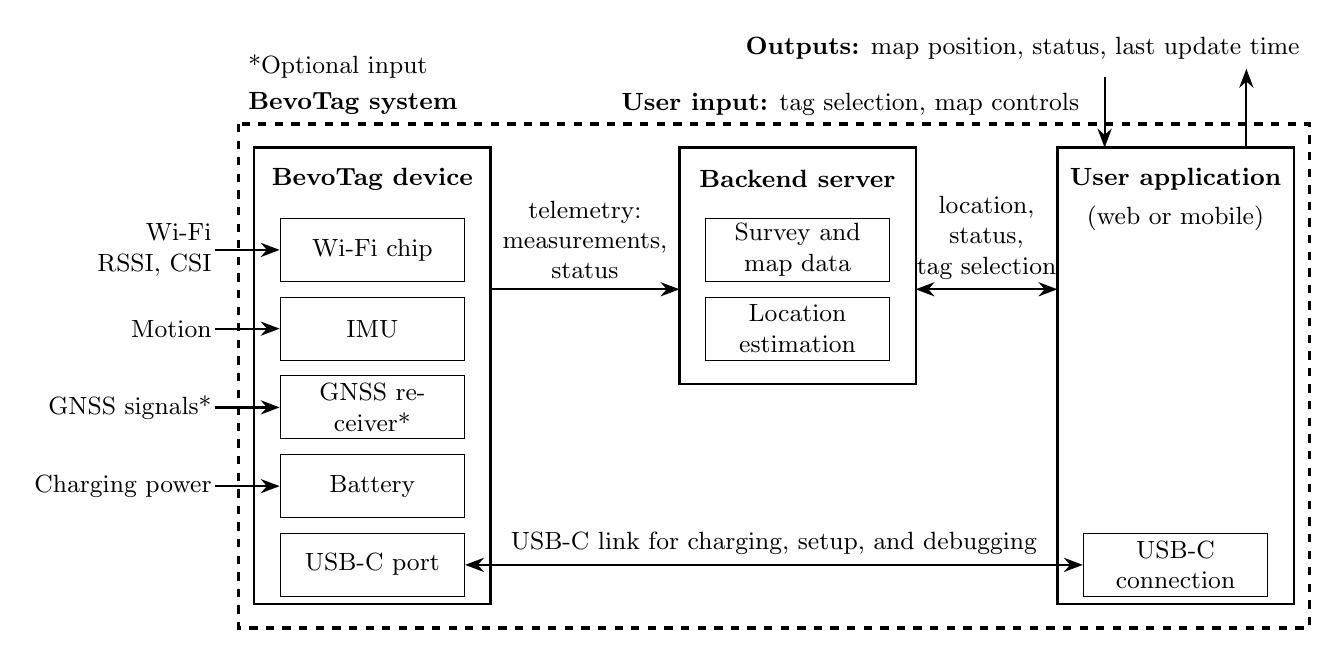
\begin{tikzpicture}[
    font=\small, >={Stealth[length=2.4mm]},
    comp/.style={draw, thick},
    sub/.style={draw, align=center, text width=2.2cm, minimum height=0.8cm, inner sep=2pt},
    ttl/.style={font=\small\bfseries, align=center},
    io/.style={align=right, text width=2.3cm, inner sep=1pt, anchor=east}]
  % Component outlines (x in cm; the figure spans the 16.5-cm text width)
  \draw[comp] (3.0,0) rectangle (6.0,-5.8);    % device
  \draw[comp] (8.4,0) rectangle (11.4,-3.0);   % server
  \draw[comp] (13.2,0) rectangle (16.2,-5.8);  % application
  \draw[very thick, dashed] (2.8,0.3) rectangle (16.4,-6.1);
  \node[ttl, anchor=south west] at (2.8,0.3) {BevoTag system};

  % BevoTag device
  \node[ttl] at (4.5,-0.4) {BevoTag device};
  \node[sub] (wifi) at (4.5,-1.3) {Wi-Fi chip};
  \node[sub] (imu)  at (4.5,-2.3) {IMU};
  \node[sub] (gnss) at (4.5,-3.3) {GNSS receiver*};
  \node[sub] (bat)  at (4.5,-4.3) {Battery};
  \node[sub] (usb1) at (4.5,-5.3) {USB-C port};

  % Backend server
  \node[ttl] at (9.9,-0.4) {Backend server};
  \node[sub] (mapd) at (9.9,-1.3) {Survey and map data};
  \node[sub] (proc) at (9.9,-2.3) {Location estimation};

  % User application
  \node[ttl] at (14.7,-0.4) {User application};
  \node at (14.7,-0.9) {(web or mobile)};
  \node[sub] (usb2) at (14.7,-5.3) {USB-C connection};

  % Inputs
  \node[io] (in1) at (2.5,-1.3) {Wi-Fi RSSI, CSI};
  \node[io] (in2) at (2.5,-2.3) {Motion};
  \node[io] (in3) at (2.5,-3.3) {GNSS signals*};
  \node[io] (in4) at (2.5,-4.3) {Charging power};
  \draw[->, thick] (in1.east) -- (wifi.west);
  \draw[->, thick] (in2.east) -- (imu.west);
  \draw[->, thick] (in3.east) -- (gnss.west);
  \draw[->, thick] (in4.east) -- (bat.west);

  % Links between components
  \draw[->, thick] (6.0,-1.8) -- node[above, align=center] {telemetry:\\measurements,\\status} (8.4,-1.8);
  \draw[<->, thick] (11.4,-1.8) -- node[above, align=center] {location,\\status,\\tag selection} (13.2,-1.8);
  \draw[<->, thick] (usb1.east) -- node[above] {USB-C link for charging, setup, and debugging} (usb2.west);

  % User input and outputs
  \draw[->, thick] (13.8,0.9) -- (13.8,0);
  \node[align=right, anchor=east] at (13.6,0.55) {\textbf{User input:} tag selection, map controls};
  \draw[->, thick] (15.6,0) -- (15.6,1.0);
  \node[align=right, anchor=south east] at (16.4,1.0) {\textbf{Outputs:} map position, status, last update time};

  % Note
  \node[anchor=south west, font=\small] at (2.8,0.75) {*Optional input};
\end{tikzpicture}
\caption{BevoTag Input and Output Diagram}
\label{fig:io}
\end{figure}

Table~\ref{tab:io} lists each input and output in Figure~\ref{fig:io} with its expected range and
units. The Wi-Fi chip must measure signals as weak as $-100$~dBm, and the tag must send telemetry
at least every 10~s while it moves, so that the application can show each new estimate within 1~s
of its arrival. GNSS appears only as an optional input for open outdoor areas.

\begin{table}[H]
\caption{BevoTag Input and Output Specifications}
\label{tab:io}
\centering
\begin{spectable}
\begin{tabularx}{\linewidth}{@{}L{1.75in} Y L{2.0in}@{}}
\toprule
\textbf{Input/Output} & \textbf{Description} & \textbf{Value or Range} \\
\midrule
Wi-Fi RSSI input & Strength of each Wi-Fi signal & $-100$ to $-30$~dBm \\
Wi-Fi CSI input & Amplitude and phase per sub-channel \cite{espcsi} & Up to 64 sub-channels \\
Acceleration input & Linear acceleration from the IMU & $\pm 8$~g \\
Angular rate input & Rotation rate from the IMU & $\pm 1000$ degrees/s \\
GNSS input (optional) & Satellite position outdoors & Latitude and longitude \\
Charging power input & Power that charges the battery & 5~V through USB-C \\
User input & Tag selection and map controls & Up to 5 tags per user \\
Telemetry & Data sent from tag to server & At most 10~s between reports \\
Location output & Estimated position of the tag & Latitude, longitude, and floor \\
Timestamp output & Time of the latest estimate & Resolution of 1~s \\
Device status output & Battery level and connectivity & 0 to 100\% charge; online or offline \\
Display refresh output & Time to show a new estimate & At most 1~s \\
\bottomrule
\end{tabularx}
\end{spectable}
\end{table}

\subsubsection{User Interface Specifications}
The user application must let a user select a tag, see its estimated location and the time of
that estimate on a 3D campus map, and check its status, and it must accept a direct USB-C
connection to a tag for configuration and debugging. Table~\ref{tab:ui} sets a value for each of
these requirements. The most important is the location display, which must show each new estimate
within 1~s of its arrival. The initial implementation may be either a web or a mobile application,
provided that it meets every requirement in the table.

\begin{table}[H]
\caption{User Interface Specifications}
\label{tab:ui}
\centering
\begin{spectable}
\begin{tabularx}{\linewidth}{@{}L{1.4in} Y L{2.4in}@{}}
\toprule
\textbf{Interface} & \textbf{Requirement} & \textbf{Value or Criterion} \\
\midrule
Device location & Show the tag on a 3D campus map & Building, floor, and position, within 1~s of each estimate \\
Device selection & Select the tag to monitor & Up to 5 tags per user \\
Last update time & Show when the position was estimated & Date and time to 1~s \\
Device status & Show battery level and connectivity & Battery percentage; online or offline \\
Map interaction & Pan, zoom, and change floors & Response within 1~s of each input \\
USB-C connection & Configure and debug a connected tag & Tag recognized within 5~s \\
\bottomrule
\end{tabularx}
\end{spectable}
\end{table}

\subsubsection{Operating Environment Specifications}
BevoTag must operate in the physical conditions of the surveyed campus zones and within the
computing and network environment that the university and the team provide, and
Table~\ref{tab:env} on the next page sets both. The test zones define the physical conditions: walls and floors that
block signals, pedestrian traffic, temperatures from 0 to 40~\textdegree C, and a carried tag that
changes orientation and moves at up to 5~m/s. The computing and network environment matters because
most of BevoTag's function is software. The tag must fit within a microcontroller's memory and join
the utexas-iot network, and its telemetry must be encrypted in transit. The backend must run on a
Linux server reachable from campus, and the application must run in current browsers or on current
phones.

\begin{table}[H]
\caption{Operating Environment Specifications}
\label{tab:env}
\centering
\begin{spectable}
\begin{tabularx}{\linewidth}{@{}L{1.45in} Y L{2.2in}@{}}
\toprule
\textbf{Condition} & \textbf{Description} & \textbf{Value or Criterion} \\
\midrule
\multicolumn{3}{@{}l}{\textit{Physical environment}} \\
Deployment area & Surveyed indoor and outdoor zones, beginning with EER & Surveyed test zones only \\
Radio environment & Signals arrive directly or only after reflection or obstruction & Line of sight and blocked, indoors and outdoors \\
Temperature & Ambient temperature for correct operation & 0 to 40~\textdegree C \\
User motion & Speed of the person carrying the tag & 0 to 5~m/s \\
\midrule
\multicolumn{3}{@{}l}{\textit{Computing and network environment}} \\
Tag processor & Battery-powered microcontroller with integrated Wi-Fi & At most 512~KB of on-chip RAM for firmware \\
Tag network & Campus network that carries telemetry & utexas-iot at 2.4~GHz, WPA2 with AES, device registered by hardware address \cite{utiot} \\
Data transport & Protection of telemetry between tag and server & TLS 1.2 or later \\
Backend host & Server that receives telemetry and serves the application & Linux virtual machine reachable from campus, with at least 2 CPU cores and 4~GB of memory \\
Application platform & Devices that run the user application & Current Chrome, Firefox, and Safari browsers, or iOS~17 and Android~13 and later \\
\bottomrule
\end{tabularx}
\end{spectable}
\end{table}

\subsubsection{Performance Specifications}
Table~\ref{tab:perf} on the next page sets the targets that define useful tracking: accuracy, timeliness, battery
life, and size and cost. Published Wi-Fi positioning systems show that meter-level accuracy is
achievable but that results vary widely with the sensing method and the radio environment
\cite{rssi}, so the team defines every target as a repeatable measurement. The team will measure
accuracy at surveyed points whose true positions it has recorded independently of BevoTag's
estimate, in stationary and moving trials indoors and outdoors. It will repeat the trials at
different times of day to capture changing conditions such as pedestrian traffic.

\begin{table}[H]
\caption{Performance Specifications}
\label{tab:perf}
\centering
\begin{spectable}
\begin{tabularx}{\linewidth}{@{}L{1.7in} Y L{1.0in} L{0.6in}@{}}
\toprule
\textbf{Parameter} & \textbf{Description} & \textbf{Value or Range} & \textbf{Units} \\
\midrule
Median position error & Median horizontal distance between estimated and true position during trials & $<5$ & m \\
Room identification & Fraction of trials in which the tag is placed in the correct surveyed room or region & $>90$ & \% \\
Floor identification & Fraction of indoor trials in which the tag is placed on the correct floor & $>95$ & \% \\
Update interval & Maximum time between location estimates while the tag moves & $\leq 10$ & s \\
End-to-end latency & Maximum time from a location estimate to its display in the application & $<5$ & s \\
Time to first fix & Maximum time from startup to the first usable position estimate & $<30$ & s \\
IMU sampling rate & Accelerometer and gyroscope sampling rate during active tracking & $\geq 100$ & Hz \\
Battery life & Operating time on one charge at one location report per minute & $\geq 24$ & h \\
Tag size & Largest dimensions of the tag in its enclosure & $\leq 80 \times 50 \times 25$ & mm \\
Tag mass & Mass of the tag with battery and enclosure & $\leq 100$ & g \\
Parts cost & Cost of components for one prototype tag & $\leq 50$ & US\$ \\
\bottomrule
\end{tabularx}
\end{spectable}
\end{table}

%----------------------------------------------------------------------------------------------------
\section{Team Organization}
%----------------------------------------------------------------------------------------------------
The five-member team has organized itself into two sub-teams under a Project Lead: Embedded
Hardware and Firmware, which builds the tag, and Localization and Application Software, which turns
measurements into a location and shows it to the user. Each member's assignment matches that
member's coursework and experience, and all members share integration, testing, and documentation.
The team coordinates through Discord and GitHub, finishes work 48~hours before each course
deadline, reviews all work before submission, and resolves disputes with evidence and a majority
vote.

\subsection{Project Roles}
The team divided its work along the boundary between the tag and the software that interprets the
tag's data. The hardware and firmware sub-team owns everything that collects measurements, and the
software sub-team owns everything that turns measurements into a displayed location. The Project
Lead and the Documentation Lead coordinate the work that crosses that boundary.

\subsubsection{Sub-Teams}
The Embedded Hardware and Firmware sub-team, Esteban Martinez and Li Shi, is responsible for the
tag itself. It will first build a data logger for feasibility experiments and Wi-Fi survey
collection, then integrate the required processing on the tag and evaluate measurement
reliability, execution time, memory use, and power consumption. The Localization and Application
Software sub-team, Andrew Yin and Abhirit Das, is responsible for turning measurements into a
location and presenting it to the user. Its work spans survey data processing, the
position-estimation pipeline, the backend that receives and manages tag data, and the user
application. The two sub-teams will integrate the tag, the positioning software, and the
application together, and all members will take part in system testing.

\subsubsection{Personnel and Team-Wide Roles}
Each member's assignment draws on specific coursework and experience, and Table~\ref{tab:roles} on the next page
summarizes these assignments. Two members also hold team-wide roles. Ethan Chua serves as Project
Lead, and Andrew Yin serves as Documentation Lead, responsible for checking every submission
against the ECE Style Guide before the team submits it.

Ethan Chua brings positioning research experience from the UT Radionavigation Laboratory, project
experience from Texas Aerial Robotics, and signal processing preparation from ECE~351M, Digital
Signal Processing. As Project Lead, Ethan will coordinate milestones, track progress, lead
integration testing, and serve as the primary contact with Dr.\ Vikalo and the Technical TA.

Esteban Martinez and Li Shi have completed ECE~445L, Embedded Systems Design Lab; ECE~422C,
Software Design and Implementation~II; and ECE~360C, Algorithms. Both have embedded systems
experience through Texas Aerial Robotics and industry internships. Their
assignments divide the tag between them. Esteban will lead component selection, power-system
design, hardware integration, and electrical testing, and Li will lead firmware development,
including Wi-Fi CSI and RSSI capture, IMU sampling, measurement timestamping, and network
communication.

Andrew Yin and Abhirit Das have completed the same three courses, and each brings application experience
that matches one half of the software sub-team's work. Andrew's experience in mobile application
development and machine learning supports Andrew's work on Wi-Fi survey processing, position
estimation, sensor fusion, and backend development. Abhirit's experience in web application
development and in profiling machine-learning deployment tools at NXP Semiconductors prepares
Abhirit to develop and test the user application.

\begin{table}[!htp]
\caption{Project Responsibilities}
\label{tab:roles}
\centering
\begin{spectable}
\begin{tabularx}{\linewidth}{@{}L{0.95in} L{1.45in} Y L{1.3in} L{1.0in}@{}}
\toprule
\textbf{Member} & \textbf{Sub-Team or Role} & \textbf{Planned Contributions} & \textbf{Areas of Expertise} & \textbf{Related Coursework} \\
\midrule
Ethan Chua & Project Lead & Coordination, integration, verification & RF positioning, GNSS, signal processing & ECE 351M \\
Esteban Martinez & Embedded Hardware and Firmware & Components, power system, hardware integration & Embedded hardware design & ECE 445L, 422C, 360C \\
Li Shi & Embedded Hardware and Firmware & Firmware, sensor drivers, Wi-Fi communication & Embedded firmware design & ECE 445L, 422C, 360C \\
Andrew Yin & Localization and Application Software; Documentation Lead & Survey processing, localization, backend & Mobile development, machine learning & ECE 445L, 422C, 360C \\
Abhirit Das & Localization and Application Software & User application, map and status display & Web development, machine-learning deployment & ECE 445L, 422C, 360C \\
\bottomrule
\end{tabularx}
\end{spectable}
\end{table}

\subsection{Team Policies}
The team's policies set how members communicate, what they owe one another, and how the team
decides questions and resolves conflict. Members use Discord for daily communication and GitHub for
code and task tracking, attend two team meetings each week and a mentor meeting every two weeks,
and finish work 48~hours before each course deadline. They review one another's work and settle
disagreements with evidence and a majority vote. The team will revisit these policies at the end
of the semester as it prepares for detailed design.

\subsubsection{Project Management Tools}
The team coordinates through four shared platforms, each with a defined purpose. Discord is the
primary communication channel, with separate channels for general coordination, each sub-team, and
meeting logistics so that discussions stay organized and searchable. A shared Google Calendar holds
meeting times, course deadlines, and internal milestones. A shared GitHub repository keeps
firmware, application code, data-processing scripts, and circuit board and enclosure designs under
version control, and GitHub Issues and a GitHub Projects board record each task's owner, due date,
and status. A shared Google Drive folder stores reports, meeting notes, and survey data. The
Project Lead handles email with Dr.\ Vikalo and the Technical TA and copies the full team, so every
member receives the same guidance.

\subsubsection{Team Expectations}
Members expect one another to communicate promptly, attend meetings prepared, review one another's
work, and finish early. These expectations give every member the same standard for accountability.

Members answer direct questions on Discord within 24~hours on weekdays and flag time-sensitive
issues, such as a blocked task or an approaching deadline, by mentioning the affected members
directly. The team meets twice a week and meets with Dr.\ Vikalo every two weeks. Members attend
every meeting having reviewed the agenda and notify the team on Discord at least 24~hours before
an unavoidable absence. Members who miss a meeting read the notes and follow up on the action items
assigned to them.

Every deliverable must meet the standard that the team would present to its mentor. A second
member reviews every pull request before it is merged, checks every circuit board design before
the team orders boards, and proofreads every written section against the ECE Style Guide. At the
start of each meeting, members report what they completed, what they plan to do next, and any
blockers, and the Project Lead records these updates and keeps the Projects board current.

Internal deadlines fall at least 48~hours before each course deadline so that the team has time to
integrate, review, and revise its work. Members who expect to miss an internal deadline tell the
team at least 48~hours in advance, so that the team can re-scope or redistribute the work.

\subsubsection{Conflict Resolution}
The team will make decisions by vote after research, settle technical disputes with tests, mediate
personal conflicts, and respond to missed responsibilities in escalating steps. Each process ends
with a clear point of escalation to the Technical TA or the course instructor.

The team makes significant decisions, such as selecting a positioning approach, choosing
components, or changing the project scope, by majority vote after researching the options. The
members most familiar with the question present the trade-offs of each option, supported by
datasheets, published results, cost estimates, or the team's own measurements, and the Project
Lead records the outcome and its rationale in the meeting notes. Each sub-team makes decisions that
affect only its own work and reports them at the next meeting. When the two members of a sub-team
disagree, the Project Lead breaks the tie.

The team settles technical disagreements with data. Where practical, it runs a quick test or trade
study against the performance specifications in Table~\ref{tab:perf} before voting. It brings any
unresolved disagreement that poses significant risk to the project to Dr.\ Vikalo or the Technical
TA.

Members first address interpersonal conflicts privately with one another. If that conversation
does not resolve the issue, an uninvolved member mediates. The team escalates any conflict that it
cannot resolve internally to the Technical TA or the course instructor.

The team responds to missed responsibilities in escalating steps. The Project Lead first raises a
missed commitment privately with the member to understand the cause and agree on a recovery plan.
The team discusses repeated missed deadlines or meetings at a team meeting and records the
corrective actions in the notes. If the problem continues, the team will notify the Technical TA
and the course instructor and will report each member's contributions accurately in peer
evaluations.

%----------------------------------------------------------------------------------------------------
\section{Conclusion}
%----------------------------------------------------------------------------------------------------
This Project Definition establishes what the BevoTag team must build and how the team will work
together to build it. Satellite positioning fails inside buildings, and existing tags depend on
other people's phones, so the team will build a low-cost tag that locates an item on campus by
matching Wi-Fi measurements against a building survey and fusing them with motion-sensor data. The
design must place an item within a median of 5~m and in the correct room in more than 90\% of
trials, within the limits that radio, data-security, and battery standards and the team's ethical
commitments set. Two sub-teams under a Project Lead will carry out the work.

The problem matters beyond lost laptops, because reliable positioning where satellite signals fail
underlies many location-aware services, and the project's outcome depends on three risks. The tag
must capture CSI on low-power hardware, room-level accuracy depends on careful building surveys,
and campus network coverage and access policies may limit where the tag can operate. If CSI
capture proves unreliable, signal-strength fingerprinting fused with motion data remains a
fallback at reduced accuracy. With that fallback and the team's experience in embedded systems,
positioning research, and software development, a working prototype within a few surveyed
buildings is a realistic outcome.

Next, the team will confirm the specification targets with Dr.\ Vikalo, complete a data logger for
initial Wi-Fi and IMU measurements, and survey EER as the first test building. It will then refine
the system block diagram and component selection, and each member will plan an individual risk
reduction activity in that member's area of the design.

%----------------------------------------------------------------------------------------------------
% REFERENCES (IEEE style, Style Guide 3.2): single-spaced entries, an empty line between entries.
%----------------------------------------------------------------------------------------------------
\renewcommand{\refname}{References}
\makeatletter
\renewenvironment{thebibliography}[1]
  {\section{\refname}%
   \setstretch{1.0}%
   \list{\@biblabel{\@arabic\c@enumiv}}%
        {\settowidth\labelwidth{\@biblabel{#1}}%
         \setlength{\leftmargin}{0.5in}%
         \setlength{\labelsep}{\dimexpr0.5in-\labelwidth\relax}%
         \setlength{\itemsep}{\baselineskip}%
         \setlength{\parsep}{0pt}%
         \setlength{\topsep}{0pt}%
         \usecounter{enumiv}%
         \renewcommand\theenumiv{\@arabic\c@enumiv}}%
   \RaggedRight}
  {\endlist}
\makeatother

\begin{thebibliography}{10}
\bibitem{airtag}
Apple Inc. (2026). \emph{AirTag} [Online]. Available: \url{https://www.apple.com/airtag/}.

\bibitem{yoder}
J. E. Yoder and T. E. Humphreys, ``Low-cost inertial aiding for deep-urban tightly coupled
multi-antenna precise GNSS,'' \emph{NAVIGATION}, vol.~70, no.~1, art.~no.~navi.561, Mar. 2023,
doi: 10.33012/navi.561.

\bibitem{imu}
O. J. Woodman, ``An introduction to inertial navigation,'' Comput. Lab., Univ. Cambridge,
Cambridge, U.K., Tech. Rep. UCAM-CL-TR-696, Aug. 2007, doi: 10.48456/tr-696.

\bibitem{gps}
National Coordination Office for Space-Based Positioning, Navigation, and Timing. (n.d.).
\emph{Space Segment} [Online]. Available: \url{https://www.gps.gov/space-segment}.

\bibitem{smarttag}
Samsung Electronics Canada. (n.d.). \emph{Galaxy SmartTag2} [Online]. Available:
\url{https://www.samsung.com/ca/business/mobile-accessories/galaxy-smarttag2-white-ei-t5600bwegca/}.

\bibitem{hechan}
S. He and S.-H. G. Chan, ``Wi-Fi fingerprint-based indoor positioning: Recent advances and
comparisons,'' \emph{IEEE Commun. Surveys Tuts.}, vol.~18, no.~1, pp.~466--490, 2016,
doi: 10.1109/COMST.2015.2464084.

\bibitem{rssi}
A. S. Yaro, F. Maly, and P. Prazak, ``A survey of the performance-limiting factors of a
2-dimensional RSS fingerprinting-based indoor wireless localization system,'' \emph{Sensors},
vol.~23, no.~5, art.~no.~2545, Feb. 2023, doi: 10.3390/s23052545.

\bibitem{utiot}
The University of Texas at Austin. (2025, Aug.~25). \emph{Connecting to utexas-iot Wi-Fi}
[Online]. Available: \url{https://ut.service-now.com/kb_view.do?sysparm_article=KB0017215}.

\bibitem{espcsi}
Espressif Systems. (2026). \emph{ESP-IDF Programming Guide (ESP32-S3): Wi-Fi Vendor Features}
[Online]. Available:
\url{https://docs.espressif.com/projects/esp-idf/en/stable/esp32s3/api-guides/wifi-driver/wifi-vendor-features.html}.

\bibitem{welch}
G. Welch and G. Bishop, ``An introduction to the Kalman filter,'' Dept. Comput. Sci., Univ. North
Carolina, Chapel Hill, NC, Tech. Rep. TR 95-041, Apr. 2004.

\bibitem{std80211}
\emph{IEEE Standard for Information Technology---Telecommunications and Information Exchange
between Systems---Local and Metropolitan Area Networks---Specific Requirements---Part 11:
Wireless LAN Medium Access Control (MAC) and Physical Layer (PHY) Specifications}, IEEE Standard
802.11-2020, Feb. 2021, doi: 10.1109/IEEESTD.2021.9363693.

\bibitem{fcc15}
\emph{Radio Frequency Devices}, 47 C.F.R. Part 15, 2025.

\bibitem{std1451}
\emph{IEEE Standard for a Smart Transducer Interface for Sensors and Actuators---Common Functions,
Communication Protocols, and Transducer Electronic Data Sheet (TEDS) Formats}, IEEE Standard
1451.0-2024, Jun. 2024, doi: 10.1109/IEEESTD.2024.10571828.

\bibitem{nist80088}
R. Chandramouli and E. A. Hibbard, \emph{Guidelines for Media Sanitization}, NIST Special
Publication 800-88 Rev.~2, Nat. Inst. Standards Technol., Gaithersburg, MD, Sept. 2025,
doi: 10.6028/NIST.SP.800-88r2.

\bibitem{fips1403}
\emph{Security Requirements for Cryptographic Modules}, FIPS PUB 140-3, Nat. Inst. Standards
Technol., Gaithersburg, MD, Mar. 2019, doi: 10.6028/NIST.FIPS.140-3.

\bibitem{iec62133}
\emph{Secondary Cells and Batteries Containing Alkaline or Other Non-Acid Electrolytes---Safety
Requirements for Portable Sealed Secondary Cells, and for Batteries Made from Them, for Use in
Portable Applications---Part 2: Lithium Systems}, IEC Standard 62133-2:2017, Feb. 2017.

\bibitem{utaup}
The University of Texas at Austin Information Security Office. (2019, Aug.~28). \emph{Acceptable
Use Policy for University Students} [Online]. Available:
\url{https://security.utexas.edu/policies/aup}.
\end{thebibliography}

%----------------------------------------------------------------------------------------------------
% APPENDIX A (Style Guide 2.7): divider page with the title one-third down, content on the next page.
% Page numbers continue from the body.
%----------------------------------------------------------------------------------------------------
\clearpage
\vspace*{0.20\textheight}
\begin{center}
\textbf{APPENDIX A -- APPLICABLE STANDARDS}
\end{center}
\clearpage

The standards and policies in this appendix require BevoTag to use a Wi-Fi chip that exposes CSI
and a pre-certified radio module, to separate its sensor drivers from its estimation code, to
encrypt its telemetry and erase its memory on reset, to use a certified and protected lithium
battery, and to use the campus network only as an ordinary client. Each section below gives the
relevant clauses in a table, states their effect on the design, and names the method the team will
use to verify compliance.

\subsection{IEEE 802.11: Wi-Fi Physical and MAC Layers}
IEEE 802.11 \cite{std80211} determines both how BevoTag can measure CSI and how it may join campus
networks. Table~\ref{tab:a80211} shows that the physical-layer clauses decide which chips can
report CSI, whereas the frame, management, and security clauses decide how the tag listens and
authenticates. The team will verify CSI capture by comparing recorded sub-channel data against
known access-point beacons, confirm passive listening with a Wireshark capture showing no
transmissions during scans, and confirm network association through connection logs on
utexas-iot.

\begin{table}[!htp]
\caption{IEEE 802.11 Requirements Affecting BevoTag}
\label{tab:a80211}
\centering
\begin{spectable}
\begin{tabularx}{\linewidth}{@{}L{1.55in} Y Y@{}}
\toprule
\textbf{Clause} & \textbf{Requirement} & \textbf{Effect on Design} \\
\midrule
Clauses 17, 18, and 19 (OFDM, ERP, and HT PHYs) & Define the sub-carrier structure and training fields at the start of each 2.4~GHz packet & The Wi-Fi chip must expose per-sub-carrier CSI from these training fields \cite{espcsi} \\
Clause 9 (frame formats) & Defines frame headers, including the transmitter address & Firmware reads only header fields, such as the access point address \\
Clause 11 (MLME) & Defines passive and active scanning and association & Tag scans passively and associates as an ordinary client \\
Clause 12 (security) & Defines robust security network association, including pre-shared keys & Tag authenticates with the WPA2 pre-shared key that utexas-iot issues \cite{utiot} \\
\bottomrule
\end{tabularx}
\end{spectable}
\end{table}

\subsection{FCC 47 CFR Part 15: Radio Frequency Devices}
Part 15 \cite{fcc15} limits both intentional transmissions and unintended emissions from the tag's
digital circuits. As Table~\ref{tab:afcc} on the next page shows, a pre-certified Wi-Fi module already satisfies the
transmitter and restricted-band limits, which leaves the team responsible mainly for board layout
and labeling. The team will verify conducted output power on a bench spectrum analyzer and check
the board for unintended emissions with a near-field probe, rather than performing full
certification testing.

\begin{table}[!htp]
\caption{FCC Part 15 Requirements Affecting BevoTag}
\label{tab:afcc}
\centering
\begin{spectable}
\begin{tabularx}{\linewidth}{@{}L{1.55in} Y Y@{}}
\toprule
\textbf{Section} & \textbf{Requirement} & \textbf{Effect on Design} \\
\midrule
\S15.109 (unintentional radiators) & Radiated emission limits for Class B digital devices & Processor clocks, sensor buses, and power conversion need careful layout and decoupling \\
\S15.247(b) (intentional radiators) & Conducted output power of at most 1~W (30~dBm) in the 2400--2483.5~MHz band, with antenna gain up to 6~dBi & Use a pre-certified Wi-Fi module whose output stays within this limit \\
\S15.205, \S15.209, and \S15.247(d) (restricted bands) & Limits on harmonics, band-edge, and spurious emissions & Rely on the certified module's filtering and follow its antenna layout rules \\
\S15.19 and \S15.212 (labeling) & Part 15 compliance statement and ``Contains FCC ID'' label for a modular radio & Enclosure carries the compliance statement and the module's FCC ID \\
\S15.21 (information to user) & Warning that unapproved changes void the user's authority to operate & Documentation includes the required warning \\
\bottomrule
\end{tabularx}
\end{spectable}
\end{table}

\subsection{IEEE 1451: Smart Transducer Interface}
IEEE 1451.0 \cite{std1451} guides how the firmware separates sensor hardware from the processing
that uses its data. Table~\ref{tab:a1451} shows that the team will adopt the standard's data model
and data sheet structure rather than its full command set, which would use more memory than the
tag can spare. The team will check compliance through firmware review and unit tests confirming
that calibration data load correctly at startup.

\begin{table}[!htp]
\caption{IEEE 1451.0 Guidelines Affecting BevoTag}
\label{tab:a1451}
\centering
\begin{spectable}
\begin{tabularx}{\linewidth}{@{}L{1.55in} Y Y@{}}
\toprule
\textbf{Provision} & \textbf{Guideline} & \textbf{Effect on Design} \\
\midrule
Transducer channel model & Each sensor appears to the processor as a set of standard channels & A hardware abstraction layer separates the IMU and Wi-Fi drivers from the fusion algorithm \\
Transducer electronic data sheets (TEDS) & Each sensor carries self-describing identification and calibration data & IMU scale factors and bias offsets are stored in a defined format in flash \\
Common communication functions & Sensor data and status are exchanged through defined message formats & Telemetry packets carry IMU, Wi-Fi, and battery data in a defined format \\
\bottomrule
\end{tabularx}
\end{spectable}
\end{table}

\subsection{NIST SP 800-88 and FIPS 140-3: Data Sanitization and Cryptography}
These federal guidelines \cite{nist80088}, \cite{fips1403} govern how the tag protects and erases
the credentials and location history it stores. Table~\ref{tab:anist} shows that a factory reset
will both overwrite stored data and destroy the encryption keys, and that telemetry and firmware
will follow FIPS 140-3 practices by relying only on approved algorithms; the team will not seek
formal module validation. The team will verify sanitization by reading back flash
memory through a debug probe after a factory reset, verify encryption against published NIST test
vectors, and verify secure boot by attempting to load an unsigned firmware image.

\begin{table}[!htp]
\caption{Data Security Requirements Affecting BevoTag}
\label{tab:anist}
\centering
\begin{spectable}
\begin{tabularx}{\linewidth}{@{}L{1.55in} Y Y@{}}
\toprule
\textbf{Section} & \textbf{Requirement} & \textbf{Effect on Design} \\
\midrule
SP 800-88 Clear (Sec.~3.1.1) & Protect against simple recovery through the device's normal interface, for example by a reset to factory state & Factory reset overwrites stored credentials, location history, and survey tables \\
SP 800-88 Purge by cryptographic erase (Sec.~3.2) & Sanitize the keys that encrypt stored data so the data cannot be decrypted & Reset erases the keys held in the chip's secure storage \\
FIPS 140-3 approved security functions & Use approved algorithms such as AES and SHA-256 & Telemetry encrypted with AES using the chip's hardware accelerator \\
FIPS 140-3 software and firmware security & Check firmware integrity with an approved digital signature & Secure boot accepts only signed firmware images \\
\bottomrule
\end{tabularx}
\end{spectable}
\end{table}

\subsection{IEC 62133-2: Lithium Battery Safety}
IEC 62133-2 \cite{iec62133} sets safety requirements for the lithium cell and battery that power
the tag. Table~\ref{tab:aiec} on the next page shows that its tests target the same hazards that the Ethical
Considerations identify, so the team will buy a cell already certified to the standard and add
charge and short-circuit protection on its own board. The team will verify that protection on the
bench by checking the charge cutoff voltage, the short-circuit cutoff, and the charge current
against the cell's datasheet limits.

\begin{table}[!htp]
\caption{IEC 62133-2 Requirements Affecting BevoTag}
\label{tab:aiec}
\centering
\begin{spectable}
\begin{tabularx}{\linewidth}{@{}L{1.55in} Y Y@{}}
\toprule
\textbf{Provision} & \textbf{Requirement} & \textbf{Effect on Design} \\
\midrule
Overcharge of battery & Battery must not catch fire or explode when charged beyond its limits & Charger limits voltage and current to the cell's rated values \\
External short circuit & Cell and battery must not catch fire or explode when shorted & Protection circuit disconnects the cell on overcurrent \\
Thermal abuse & Cell must withstand elevated temperature without fire or explosion & Charging stops outside the cell's rated temperature range \\
Certified cells & Cells must pass the standard's type tests & Team buys only cells certified to IEC 62133-2 \\
\bottomrule
\end{tabularx}
\end{spectable}
\end{table}

\subsection{UT Austin Acceptable Use Policy}
The university's acceptable use policy \cite{utaup} and its registration rules for utexas-iot
\cite{utiot} govern how the tag uses the campus network. Table~\ref{tab:aaup} on the next page shows that the
policy's limits on probing and interference match the tag's design as a passive, ordinary network
client. The team will verify
compliance by reviewing the firmware's network functions against the policy and by confirming with
a Wireshark capture that the tag sends only its own telemetry.

\begin{table}[!htp]
\caption{UT Austin Acceptable Use Policy Provisions Affecting BevoTag}
\label{tab:aaup}
\centering
\begin{spectable}
\begin{tabularx}{\linewidth}{@{}L{1.55in} Y Y@{}}
\toprule
\textbf{Provision} & \textbf{Requirement} & \textbf{Effect on Design} \\
\midrule
AUP Sec.~5.10 (scanning) & Never deliberately scan or probe an information resource without authorization & Tag listens passively and never sends probe or scanning traffic \\
AUP Sec.~5.7 (shared resources) & Do not interfere with others' use or consume a disproportionate share & Tag sends only small, periodic telemetry reports \\
utexas-iot registration \cite{utiot} & Register each device's hardware address through the university's network portal & Team registers each tag and disables address randomization \\
\bottomrule
\end{tabularx}
\end{spectable}
\end{table}

\end{document}
